\documentclass{standalone}
\usepackage{tikz}
\usetikzlibrary{patterns, positioning}
\usepackage[sfdefault]{ClearSans} %% option 'sfdefault' activates Clear Sans as the default text font
\usepackage[T1]{fontenc}

\begin{document}
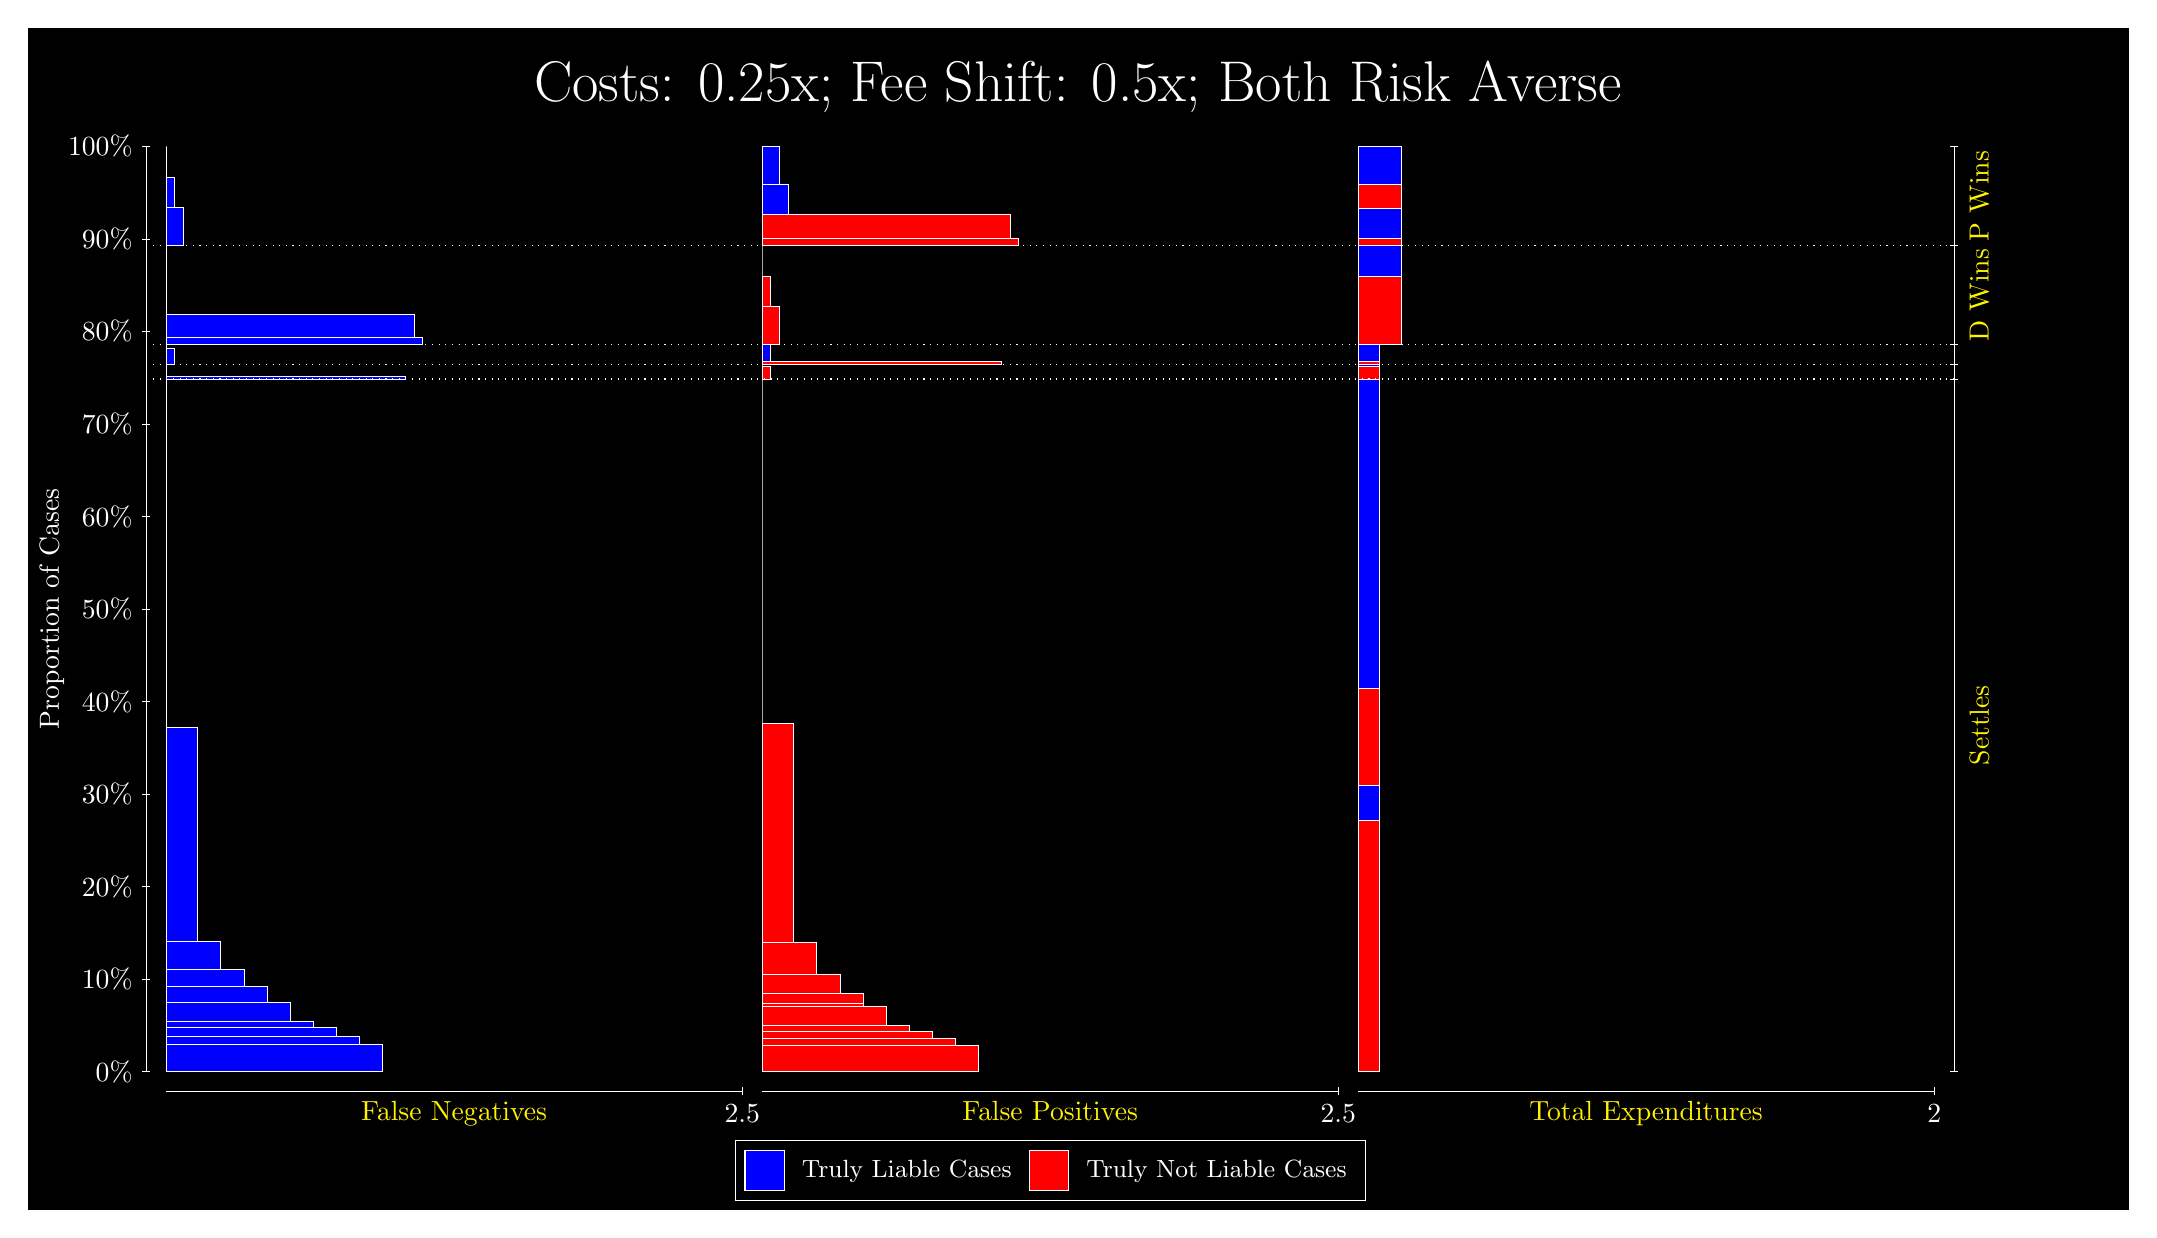
\begin{tikzpicture}
\draw[fill=black] (0,0) rectangle (26.667,15);
\draw[text=white] (0,13.5) rectangle (26.667,15) node[midway] {\huge Costs: 0.25x; Fee Shift: 0.5x; Both Risk Averse};
\draw[white, very thin] (1.5,1.75) -- (1.5,13.5);
\node[rotate=90, text=white, anchor=center] at (0.3, 7.625) {Proportion of Cases};
\draw[white, very thin] (1.45,1.75) -- (1.55,1.75);
\node[text=white, anchor=east] at (1.45, 1.75) {0\%};
\draw[white, very thin] (1.45,2.925) -- (1.55,2.925);
\node[text=white, anchor=east] at (1.45, 2.925) {10\%};
\draw[white, very thin] (1.45,4.1) -- (1.55,4.1);
\node[text=white, anchor=east] at (1.45, 4.1) {20\%};
\draw[white, very thin] (1.45,5.275) -- (1.55,5.275);
\node[text=white, anchor=east] at (1.45, 5.275) {30\%};
\draw[white, very thin] (1.45,6.45) -- (1.55,6.45);
\node[text=white, anchor=east] at (1.45, 6.45) {40\%};
\draw[white, very thin] (1.45,7.625) -- (1.55,7.625);
\node[text=white, anchor=east] at (1.45, 7.625) {50\%};
\draw[white, very thin] (1.45,8.8) -- (1.55,8.8);
\node[text=white, anchor=east] at (1.45, 8.8) {60\%};
\draw[white, very thin] (1.45,9.975) -- (1.55,9.975);
\node[text=white, anchor=east] at (1.45, 9.975) {70\%};
\draw[white, very thin] (1.45,11.15) -- (1.55,11.15);
\node[text=white, anchor=east] at (1.45, 11.15) {80\%};
\draw[white, very thin] (1.45,12.325) -- (1.55,12.325);
\node[text=white, anchor=east] at (1.45, 12.325) {90\%};
\draw[white, very thin] (1.45,13.5) -- (1.55,13.5);
\node[text=white, anchor=east] at (1.45, 13.5) {100\%};

\draw[white, very thin] (24.457,1.75) -- (24.457,13.5);
\draw[white, very thin] (24.407,1.75) -- (24.507,1.75);
\node[anchor=west] at (24.407, 1.75) {};
\draw[white, very thin] (24.407,10.545) -- (24.507,10.545);
\node[anchor=west] at (24.407, 10.545) {};
\draw[white, very thin] (24.407,10.732) -- (24.507,10.732);
\node[anchor=west] at (24.407, 10.732) {};
\draw[white, very thin] (24.407,10.98) -- (24.507,10.98);
\node[anchor=west] at (24.407, 10.98) {};
\draw[white, very thin] (24.407,12.238) -- (24.507,12.238);
\node[anchor=west] at (24.407, 12.238) {};
\draw[white, very thin] (24.407,13.5) -- (24.507,13.5);
\node[anchor=west] at (24.407, 13.5) {};

\draw[white, very thin, fill=blue] (1.75,1.75) rectangle (4.4946,2.101);
\draw[white, very thin, fill=blue] (1.75,2.101) rectangle (4.2018,2.1996);
\draw[white, very thin, fill=blue] (1.75,2.1996) rectangle (3.9091,2.3072);
\draw[white, very thin, fill=blue] (1.75,2.3072) rectangle (3.6163,2.3885);
\draw[white, very thin, fill=blue] (1.75,2.3885) rectangle (3.3236,2.629);
\draw[white, very thin, fill=blue] (1.75,2.629) rectangle (3.0308,2.8336);
\draw[white, very thin, fill=blue] (1.75,2.8336) rectangle (2.738,3.0505);
\draw[white, very thin, fill=blue] (1.75,3.0505) rectangle (2.4453,3.4095);
\draw[white, very thin, fill=blue] (1.75,3.4095) rectangle (2.1525,6.1252);
\draw[white, very thin, fill=red] (1.75,6.1252) rectangle (1.75,10.545);
\draw[white, very thin, fill=blue] (1.75,10.545) rectangle (4.7873,10.576);
\draw[white, very thin, fill=red] (1.75,10.576) rectangle (1.75,10.732);
\draw[white, very thin, fill=blue] (1.75,10.732) rectangle (1.8598,10.94);
\draw[white, very thin, fill=red] (1.75,10.94) rectangle (1.75,10.98);
\draw[white, very thin, fill=blue] (1.75,10.98) rectangle (5.0069,11.071);
\draw[white, very thin, fill=blue] (1.75,11.071) rectangle (4.8971,11.372);
\draw[white, very thin, fill=red] (1.75,11.372) rectangle (1.75,12.238);
\draw[white, very thin, fill=blue] (1.75,12.238) rectangle (1.9696,12.726);
\draw[white, very thin, fill=blue] (1.75,12.726) rectangle (1.8598,13.108);
\draw[white, very thin, fill=red] (1.75,13.108) rectangle (1.75,13.5);
\draw[white, very thin, fill=red] (9.3189,1.75) rectangle (12.063,2.0881);
\draw[white, very thin, fill=red] (9.3189,2.0881) rectangle (11.771,2.1689);
\draw[white, very thin, fill=red] (9.3189,2.1689) rectangle (11.478,2.2554);
\draw[white, very thin, fill=red] (9.3189,2.2554) rectangle (11.185,2.3425);
\draw[white, very thin, fill=red] (9.3189,2.3425) rectangle (10.892,2.5798);
\draw[white, very thin, fill=red] (9.3189,2.5798) rectangle (10.6,2.6134);
\draw[white, very thin, fill=red] (9.3189,2.6134) rectangle (10.6,2.7411);
\draw[white, very thin, fill=red] (9.3189,2.7411) rectangle (10.307,2.9843);
\draw[white, very thin, fill=red] (9.3189,2.9843) rectangle (10.014,3.3864);
\draw[white, very thin, fill=red] (9.3189,3.3864) rectangle (9.7214,6.1694);
\draw[white, very thin, fill=blue] (9.3189,6.1694) rectangle (9.3189,10.545);
\draw[white, very thin, fill=red] (9.3189,10.545) rectangle (9.4287,10.701);
\draw[white, very thin, fill=blue] (9.3189,10.701) rectangle (9.3189,10.732);
\draw[white, very thin, fill=red] (9.3189,10.732) rectangle (12.356,10.773);
\draw[white, very thin, fill=blue] (9.3189,10.773) rectangle (9.4287,10.98);
\draw[white, very thin, fill=red] (9.3189,10.98) rectangle (9.5384,11.466);
\draw[white, very thin, fill=red] (9.3189,11.466) rectangle (9.4287,11.846);
\draw[white, very thin, fill=blue] (9.3189,11.846) rectangle (9.3189,12.238);
\draw[white, very thin, fill=red] (9.3189,12.238) rectangle (12.576,12.33);
\draw[white, very thin, fill=red] (9.3189,12.33) rectangle (12.466,12.631);
\draw[white, very thin, fill=blue] (9.3189,12.631) rectangle (9.6482,13.012);
\draw[white, very thin, fill=blue] (9.3189,13.012) rectangle (9.5384,13.5);
\draw[white, very thin, fill=red] (16.888,1.75) rectangle (17.162,4.9351);
\draw[white, very thin, fill=blue] (16.888,4.9351) rectangle (17.162,5.3847);
\draw[white, very thin, fill=red] (16.888,5.3847) rectangle (17.162,6.619);
\draw[white, very thin, fill=blue] (16.888,6.619) rectangle (17.162,10.545);
\draw[white, very thin, fill=red] (16.888,10.545) rectangle (17.162,10.701);
\draw[white, very thin, fill=blue] (16.888,10.701) rectangle (17.162,10.732);
\draw[white, very thin, fill=red] (16.888,10.732) rectangle (17.162,10.773);
\draw[white, very thin, fill=blue] (16.888,10.773) rectangle (17.162,10.98);
\draw[white, very thin, fill=red] (16.888,10.98) rectangle (17.437,11.846);
\draw[white, very thin, fill=blue] (16.888,11.846) rectangle (17.437,12.238);
\draw[white, very thin, fill=red] (16.888,12.238) rectangle (17.437,12.33);
\draw[white, very thin, fill=blue] (16.888,12.33) rectangle (17.437,12.712);
\draw[white, very thin, fill=red] (16.888,12.712) rectangle (17.437,13.012);
\draw[white, very thin, fill=blue] (16.888,13.012) rectangle (17.437,13.5);
\draw[white, dotted] (1.5,10.545) -- (24.457,10.545);
\draw[white, dotted] (1.5,10.732) -- (24.457,10.732);
\draw[white, dotted] (1.5,10.98) -- (24.457,10.98);
\draw[white, dotted] (1.5,12.238) -- (24.457,12.238);
\draw[white, very thin] (1.75,1.5) -- (9.0689,1.5);
\node[text=yellow, anchor=north] at (5.4094, 1.5) {False Negatives};
\draw[white, very thin] (9.0689,1.45) -- (9.0689,1.55);
\node[text=white, anchor=north] at (9.0689, 1.45) {2.5};

\draw[white, very thin] (9.3189,1.5) -- (16.638,1.5);
\node[text=yellow, anchor=north] at (12.978, 1.5) {False Positives};
\draw[white, very thin] (16.638,1.45) -- (16.638,1.55);
\node[text=white, anchor=north] at (16.638, 1.45) {2.5};

\draw[white, very thin] (16.888,1.5) -- (24.207,1.5);
\node[text=yellow, anchor=north] at (20.547, 1.5) {Total Expenditures};
\draw[white, very thin] (24.207,1.45) -- (24.207,1.55);
\node[text=white, anchor=north] at (24.207, 1.45) {2};

\node[text=yellow, centered, rotate=90] at (24.777, 6.1473) {Settles};


\node[text=yellow, centered, rotate=90] at (24.777, 11.609) {D Wins};
\node[text=yellow, centered, rotate=90] at (24.777, 12.869) {P Wins};

\draw (12.978300999999998,1.5) node[draw=none] (baseCoordinate) {};
\begin{scope}[align=center]
        \matrix[scale=0.5, draw=white, below=0.5cm of baseCoordinate, nodes={draw}, column sep=0.1cm]{
            \node[rectangle, draw, minimum width=0.5cm, minimum height=0.5cm, fill=blue] {}; &
            \node[draw=none, font=\small, text=white] (B) {Truly Liable Cases}; &
            \node[rectangle, draw, minimum width=0.5cm, minimum height=0.5cm, fill=red] {}; &
            \node[draw=none, font=\small, text=white] (B) {Truly Not Liable Cases}; \\
            };
\end{scope}

\end{tikzpicture}
\end{document}